\documentclass[11pt]{article}

\usepackage[margin=0.82in]{geometry}
\usepackage[T1]{fontenc}
\usepackage[utf8]{inputenc}
\usepackage{lmodern}
\usepackage{microtype}
\usepackage{amsmath,amssymb,mathtools}
\usepackage{booktabs,longtable,array,tabularx}
\usepackage[table]{xcolor}
\usepackage{enumitem}
\usepackage{hyperref}
\usepackage{tikz}
\usepackage{pgfplots}
\usepackage[most]{tcolorbox}
\usepackage{caption}
\usepackage{float}
\usepackage{fancyhdr}
\usepackage{titlesec}

\usetikzlibrary{arrows.meta,positioning,fit,calc,shapes.geometric,decorations.pathreplacing}
\pgfplotsset{compat=1.18}

\definecolor{navy}{RGB}{24,45,75}
\definecolor{ink}{RGB}{35,49,70}
\definecolor{slate}{RGB}{79,96,119}
\definecolor{fixedblue}{RGB}{59,130,246}
\definecolor{fixedpale}{RGB}{231,240,254}
\definecolor{observedgold}{RGB}{219,151,30}
\definecolor{observedpale}{RGB}{255,245,216}
\definecolor{unknownpurple}{RGB}{132,84,194}
\definecolor{unknownpale}{RGB}{241,233,252}
\definecolor{calcteal}{RGB}{17,146,137}
\definecolor{calcpale}{RGB}{222,245,242}
\definecolor{outputgreen}{RGB}{53,139,82}
\definecolor{outputpale}{RGB}{229,245,233}
\definecolor{coral}{RGB}{226,91,78}
\definecolor{coralpale}{RGB}{253,233,230}
\definecolor{lightgray}{RGB}{245,247,250}
\definecolor{midgray}{RGB}{215,223,232}

\hypersetup{
  colorlinks=true,
  linkcolor=calcteal,
  urlcolor=fixedblue!70!black,
  citecolor=unknownpurple,
  pdftitle={ShapeMix-ATAC Simplified Explanation},
  pdfauthor={Andy Zhuang},
  pdfsubject={Progressive tutorial for the ShapeMix-ATAC Bayesian model},
  pdfkeywords={ShapeMix, ATAC-seq, Bayesian model, deconvolution, fragment length, MAP}
}

\setlength{\headheight}{14pt}
\setlength{\parindent}{0pt}
\setlength{\parskip}{0.43em}
\renewcommand{\arraystretch}{1.18}
\pagestyle{fancy}
\fancyhf{}
\lhead{ShapeMix-ATAC Simplified Explanation}
\rhead{Bayesian model tutorial}
\cfoot{\thepage}

\titleformat{\section}{\Large\bfseries\color{navy}}{\thesection}{0.65em}{}
\titleformat{\subsection}{\large\bfseries\color{calcteal}}{\thesubsection}{0.65em}{}
\titleformat{\subsubsection}{\normalsize\bfseries\color{unknownpurple}}{\thesubsubsection}{0.65em}{}

\newcolumntype{L}[1]{>{\raggedright\arraybackslash}p{#1}}
\newcolumntype{C}[1]{>{\centering\arraybackslash}p{#1}}

\newcommand{\NB}{\operatorname{NegBinomial}}
\newcommand{\Mult}{\operatorname{Multinomial}}
\newcommand{\Gam}{\operatorname{Gamma}}
\newcommand{\Pois}{\operatorname{Poisson}}
\newcommand{\E}{\mathbb{E}}
\newcommand{\Var}{\operatorname{Var}}
\newcommand{\given}{\,|\,}
\newcommand{\fixedq}[1]{\textcolor{fixedblue!75!black}{#1}}
\newcommand{\obsq}[1]{\textcolor{observedgold!80!black}{#1}}
\newcommand{\unknownq}[1]{\textcolor{unknownpurple}{#1}}
\newcommand{\calcq}[1]{\textcolor{calcteal!85!black}{#1}}
\newcommand{\outputq}[1]{\textcolor{outputgreen!85!black}{#1}}

\newtcolorbox{bigidea}{
  colback=fixedpale,
  colframe=fixedblue!75!black,
  title=Main idea,
  fonttitle=\bfseries,
  breakable
}
\newtcolorbox{newvar}[1]{
  colback=lightgray,
  colframe=navy,
  title={New symbol: #1},
  fonttitle=\bfseries,
  breakable
}
\newtcolorbox{checkpoint}{
  colback=outputpale,
  colframe=outputgreen!80!black,
  title=Pause and check,
  fonttitle=\bfseries,
  breakable
}
\newtcolorbox{watchout}{
  colback=coralpale,
  colframe=coral,
  title=Important distinction,
  fonttitle=\bfseries,
  breakable
}
\newtcolorbox{translation}{
  colback=calcpale,
  colframe=calcteal,
  title=Say the equation in words,
  fonttitle=\bfseries,
  breakable
}
\newtcolorbox{worked}[1]{
  colback=observedpale,
  colframe=observedgold,
  title=#1,
  fonttitle=\bfseries,
  breakable
}
\newtcolorbox{advanced}[1]{
  colback=white,
  colframe=slate,
  title={Advanced detail: #1},
  fonttitle=\bfseries,
  breakable
}

\begin{document}
\hypersetup{pageanchor=false}

\begin{titlepage}
\centering
\vspace*{0.25in}
{\Huge\bfseries\color{navy} ShapeMix-ATAC Simplified Explanation\par}

\end{titlepage}

\hypersetup{pageanchor=true}
\pagenumbering{roman}
\setcounter{tocdepth}{1}
\tableofcontents
\newpage
\pagenumbering{arabic}

\section{Bayesian model without fragment length bins}



\subsection{Array indices}

\begin{center}
\begin{tabular}{C{0.11\linewidth}L{0.66\linewidth}}
\toprule
Index & Meaning \\
\midrule
\(s\) & which spatial spot? \\
\(p\) & which selected genomic peak? \\
\(b\) & which parent-fragment length bin? \\
\(c\) & which reference cell type? \\
\bottomrule
\end{tabular}
\end{center}

\subsection{Array dimensions}

\begin{center}
\begin{tabular}{C{0.11\linewidth}L{0.66\linewidth}}
\toprule
Dimension & Meaning \\
\midrule
\(S\) & number of spatial spots \\
\(P\) & number of peaks \\
\(B\) & number of fragment length bins=3 \\
\(C\) & number of cell types \\
\bottomrule
\end{tabular}
\end{center}


\subsection{Symbols}

\begin{center}
\begin{tabular}{C{0.12\linewidth}L{0.40\linewidth}C{0.16\linewidth}L{0.14\linewidth}}
\toprule
Symbol & Meaning & Shape & Role \\
\midrule
\(R\) & reference peak rate & \(C\times P\) & fixed \\
\(z\) & effective abundance & \(S\times C\)  & unknown \\
\(n\) & predicted (mean) counts & \(S\times P\)  & calculated \\
\(N\) & observed total counts & \(S\times P\)  & data \\
\bottomrule
\end{tabular}
\end{center}

\subsection{Bayesian model}

\[
\underbrace{p(z\mid N)}_{\text{posterior}}
\propto
\underbrace{p(N \mid z)}_{\text{likelihood}} \cdot
\underbrace{p(z)}_{\text{prior}}
\]

The peak count total is modeled by a negative binomial:
\[
\boxed{
N\sim\NB\!\left(
\text{mean } n=z \cdot R,\;
\text{inverse-dispersion}=\phi_{\mathrm{ref}} \cdot \sum_c{z}
\right)
}
\]

where $\phi_{\mathrm{ref}}$ is a constant. $z \cdot R$ is a dot product between two
vectors: for one spot $s$ and one peak $p$, $n_{s,p}=\sum_c z_{s,c}R_{c,p}$.



Every element of $z$ has the same Gamma prior:
\[
\boxed{z\sim\Gam(\text{shape}=2,\text{rate}=1)}
\]

This is the frozen version-1 prior. It has mean 2, variance 2, and mode 1.

\begin{figure}[H]
\centering
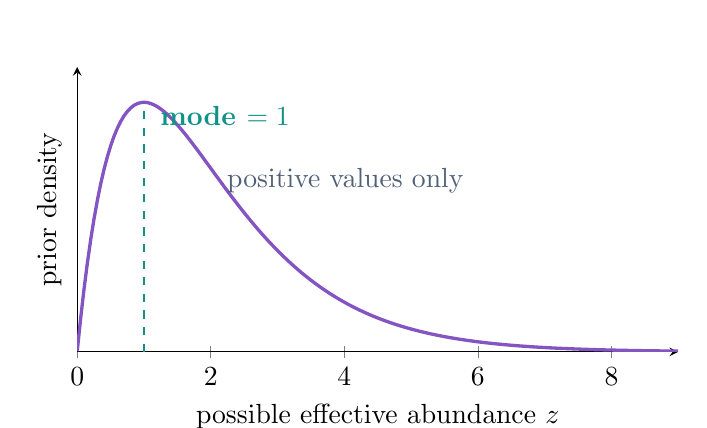
\begin{tikzpicture}
\begin{axis}[
  width=0.76\linewidth,
  height=5.2cm,
  xmin=0,xmax=9,
  ymin=0,ymax=0.42,
  xlabel={possible effective abundance \(z\)},
  ylabel={prior density},
  ytick=\empty,
  axis lines=left,
  samples=180
]
  \addplot[domain=0.001:9,very thick,unknownpurple] {x*exp(-x)};
  \addplot[dashed,calcteal,thick] coordinates {(1,0) (1,0.3679)};
  \node[anchor=south west,text=calcteal,font=\bfseries] at (axis cs:1.1,0.32) {mode \(=1\)};
  \node[anchor=south west,text=slate] at (axis cs:2.1,0.22) {positive values only};
\end{axis}
\end{tikzpicture}
\caption{The \(\Gam(2,1)\) prior is a probability density over positive effective abundance.}
\end{figure}


\section{Bayesian model for ShapeMix}

\subsection{Symbols extended to bin counts}

\begin{center}
\begin{tabular}{C{0.12\linewidth}L{0.40\linewidth}C{0.16\linewidth}L{0.14\linewidth}}
\toprule
Symbol & Meaning & Shape & Role \\
\midrule
\(R_{\mathrm{LB}}\) & reference rate per length bin & \(C\times P\times B\) & fixed \\
\(n_{\mathrm{LB}}\) & predicted (mean) bin counts & \(S\times P\times B\)  & calculated \\
\(N_{\mathrm{LB}}\) & observed bin counts & \(S\times P\times B\)  & data \\
\bottomrule
\end{tabular}
\end{center}

Summing over the three length bins recovers the totals from Section~1:
\[
R=\sum_b R_{\mathrm{LB}},
\qquad
n=\sum_b n_{\mathrm{LB}},
\qquad
N=\sum_b N_{\mathrm{LB}}.
\]

\subsection{Bayesian model}

\[
\underbrace{p(z\mid N_{\mathrm{LB}}, N)}_{\text{posterior}}
\propto
\underbrace{p(N_{\mathrm{LB}}, N \mid z)}_{\text{likelihood}} \cdot
\underbrace{p(z)}_{\text{prior}} = p(N_{\mathrm{LB}} \mid N, z) \cdot p(N \mid z) \cdot p(z)
\]

The distribution of the last two terms has already been introduced. For $p(N_{\mathrm{LB}} \mid N, z)$, it is a multinomial distribution:

\[
\boxed{
N_{\mathrm{LB}}\mid N
\sim
\Mult(N,\frac{n_{\mathrm{LB}}}{n})=\Mult(N,\frac{z \cdot R_{\mathrm{LB}}}{n})
}
\]


\iffalse
\fi

\end{document}
